
\documentclass{article}
\usepackage[utf8]{inputenc}
\usepackage[a4paper, total={7in, 8in}]{geometry}
\usepackage{braket}
\usepackage{xcolor}
\usepackage{amsmath}
\usepackage{amssymb}
\usepackage{amsfonts}
\usepackage{graphicx}
\usepackage{svg}
\usepackage{media9}
\usepackage{float}
\usepackage{tikz}
\usepackage[ruled,vlined]{algorithm2e}
\usepackage{pdfpages}
% \usepackage{biblatex} %Imports biblatex package
\usepackage{hyperref}
\usepackage{cleveref}
\hypersetup{colorlinks=true}

\usepackage[
backend=biber,
style=alphabetic,
sorting=ynt
]{biblatex}

\addbibresource{sample.bib} %Import the bibliography file

\newcommand{\commentt}[1]{\textcolor{blue}{ \textbf{[COMMENT]} #1}}
\newcommand{\ctt}[1]{\commentt{#1}}
\newcommand{\prb}[1]{ \mathbf{Pr} \left[ {#1} \right]}
\newcommand{\onotation}[1]{\(\mathcal{O} \left( {#1}  \right) \)}
\newcommand{\ona}[1]{\onotation{#1}}
\newcommand{\PSI}{{\ket{\psi}}}
\newcommand{\LESn}{\ket{\psi_n}}
\newcommand{\LESa}{\ket{\phi_n}}
\newcommand{\LESs}{\frac{1}{\sqrt{n}}\sum_{i}{\ket{\left(0^{i}10^{n-i}\right)^{n}}}}
\newcommand{\Hn}{\mathcal{H}_{n}}
% \author{David Ponarovsky}
% \date{July 2021}

\newcommand{\Ep}{\frac{1}{\sqrt{2^n}}\sum^{2^n}_{x}{ \ket{xx}}}
\newcommand{\HON}{\ket{\psi_{\text{honest}}}}
\usepackage{multicol}
% \usepackage{  }
\setlength{\columnsep}{0.6cm}


\begin{document}
    
\title{ Efficiently Trotterizing Lithium Hydride Time Eveloution Step  \\  Experimential Project  Classiq}
\author{David Ponarovsky}
\maketitle

\begin{abstract} 
In this paper, we review our experimental implementation of an algorithm for designing time evolution simulation circuits of molecules, given their Hamiltonian in the Pauli basis. Our algorithm employs several heuristics to minimize the circuit depth. We demonstrated this by taking the lithium hydride molecule as a use case and comparing the generated circuit to the one produced by the naive approach.
\end{abstract}

\begin{multicols}{2}

\section{Preamble.}
Simulation is definitely one of the core ingredients that our modern civilization relies on; the fact that one can check on their computer if their sketch for an electronic chip or plane will actually compute or fly without the need to construct and test a physical prototype both cheapens and accelerates the development process. 

Though humanity has successfully enabled an efficient simulation in a variety of regimes, there are still areas in which we don't have any other choices than performing physical experiments. Development of materials, drugs, and medicines is a good example of a processes that suffer from the lack of simulation and can last for decades. What distinguishes those areas is the fact that the mechanics theory governing them is quantum mechanics, which we have good reason to believe cannot be simulated by classical computers. Yet, quantum computers are considered to be good candidates to overcome that barrier. 

Unfortunately, our current quantum machines are extremely limited in terms of computing resources; the most advanced computers have access to no more than a few hundred qubits and suffer from a considerable amount of noise, which cause long computations resulting in nonsense. Therefore, any short-term application must be cost-efficient.

On May 2022, Classiq, a pioneering quantum computing company, launched the first (at least at that scale) competition in quantum circuits programming. The initial purpose of this work was to solve the Lithium simulation problem. In short, the problem asked to come up with a quantum circuit, restricted to only a few qubits, that progress the lithium hydride molecule in time. The winner of the competition would be the circuit with the shortest depth. We mention that our algorithm is generic and the software we have written can easily be modified for any other Hamiltonian.

The paper organized in the follow systematically manner, first in the preamble we will present the problem and talk about the general concepts which describe our specific Hamiltonian, including the quantities regime (i.e number of qubits vs number of Hamiltonians terms), the naive solution, and how mach improvement we could hope to make.     


Then in next section we review all the techniques that we have used to improve a  local gates assignment. Namely, this section deals with the question of how presenting each of the local term as subgate. 

  In contrast, the third and the forth sections reviews methods to determinate an  order which clearly superior comparing to the naive approach. The forth section presenting an concept of analyzing the "product graph" a concept which could be thought as the second order analyses of the alternate path from the third section.      
  \paragraph{The problem.} \textit{Generate a circuit, using no more than \(10\) qubits, that approximates the unitary \(e^{-iH}\) where \(H\) is the qubit Hamiltonian of a \textbf{LiH} (lithium hydride) molecule. The \textbf{LiH} Hamiltonian is composed of 276 Pauli strings, and can be found \hyperlink{LiH.html.pdf.1}{HERE}. The approximation error is defined in the next section, and should be less than \(0.1\). The circuit should be composed of the \(CX\) and single qubit gates only.}
  \paragraph{Simulation in nutshell.} Let's begin by introducing notation, adhering to standard definitions; a quantum state $\ket{\psi}$ is a vector in a Hilbert space, and a Hamiltonian is a Hermitian operator acting on that space. As physical fundamentals are not the main focus of the paper, we will merely mention, without providing justification, that a quantum state at time $t$ in the presence of a Hamiltonian $H$ is given by the relation $\ket{\psi\left( t\right)} = e^{-iHt}\ket{\psi\left( 0 \right)}$. Note that, due to the fact that $H$ is a Hermitian operator, $e^{-iHt}$ is a unitary operator.

For example, suppose that $\ket{\psi} = \ket{00}$ and $H = Z\otimes Z $. Thus, the time evolution operator is $e^{itZ\otimes Z}$. As $\ket{00}$ is an eigenstate of $H$, since $Z\otimes Z \ket{00} = \ket{00}$, we have that $\ket{\psi\left( t \right)} = e^{-it}\ket{00}$. However, if $\ket{\psi} = \ket{00} + \ket{10}$ (ignoring normalization factors), then we would have that $\ket{\psi(t)} = e^{-it}\ket{00} + e^{it}\ket{10}$.

For simulating a general Hamiltonian, recall that the Pauli matrices, along with the identity, span the space of matrices. Thus, one can assume that the Hamiltonian is given as a linear combination of Paulis. We will denote it as $H = \sum_{i}{H_{i}}$, where each of the $H_{i}$ is a Pauli product multiplied by a scalar factor.

Using the Lie-Trotter formula \cite{Lie-Trotter} 
\begin{equation*}
  \begin{split}
    e^{A+B} = \lim_{n \rightarrow \infty} (e^{A/n}e^{B/n})^n 
  \end{split}
\end{equation*}
for arbitrary matrices $A,B$, we obtain that one can apply the gates $e^{\Delta t H_{i}}$ for $1/(\Delta t)$ iterations and expect to converge to the desired product. This insight defines a circuit which we will refer to as the naive approach.

\paragraph{Naive approach.}  Before diving into the technical details, let's first review our competitor. Consider the straightforward assignment Lie-Trotter \cite{Lie-Trotter}, which handles each of the Hamiltonian terms one by one. Assume that the Hamming weight of the support of \(H_i\) is equal to \(d_i\). Thus, we need two steps to rotate each wire into the parity base (relative to the Hamiltonian) and uncompute it in the end. Then, we can apply the \(CX\) from each qubit in the support to a (arbitrary) chosen one, which will sum the wires' parity and finally propagate the sum through the \(RZ\left(\theta \Delta t \right) \) gate (rotation by the coefficient of the term and the step size). Therefore, in total we pay \(2 + 2d_i\) for each term and the whole circuit will require:
\begin{equation*}
    \begin{split}
        D^{\text{naive}}\left(n,m\right) & = \sum_{i}{2 + 2d_i} = m\sum_{i}{\frac{2 + 2d_i}{m}} = \\
        & 2m \left\Big( 1 + \mathbb{E}_{\sim i}[H] \right\Big)  
    \end{split}
\end{equation*}

Where \(D^{\text{naive}}\left(n,m\right)\) is the depth of the circuit which computes a single \( \Delta t \) step of the Lie-Trotter formula\cite{Lie-Trotter}. To gain a better understanding of what constitutes a good solution, let us assume for the moment that \( \mathbb{E}_{\sim i}[H] > 5 \). Under this assumption, the naive approach yields a circuit of depth \(\ge 2 \cdot 276 \cdot 6 \sim 3100 \). Ultimately, we will see that our solution produces a \(1759\)-depth circuit.

\paragraph{Characterize our \textbf{LiH}.} A natural question to ask is whether there exists a more efficient way to present the Hamiltonian. Although we cannot be certain that there is not, let's try to estimate how much improvement can be achieved by applying the Bravyi-Kitaev transformation \cite{Bravyi_2002} . In one sentence, Bravyi and Kitaev have shown that the ladder and annihilation operators have Pauli representations such that each operator touches at least \( \log\left(n\right) \) of the qubits. Since the Hamiltonian of molecule\footnote{Sometimes called electronic structure Hamiltonian} in the energy base has a "product" of four operators (i.e \( a^{\dagger}_{i}a^{\dagger}_{j}a_{n}a_{m} \)), we get that there may be operators in the computing base which touch \(4\log\left(n\right)\) qubits. In our case, \(n = 10 \Rightarrow 4\log\left(n\right) > n \). 
In conclusion, it seems that the known techniques for reducing the support of the terms asymptotically do not work here. This is an indication that a 10-fold improvement is unlikely. Therefore, we will aim for a 2-fold improvement over the naive approach.
\section{Single Term Heuristics.}

\paragraph{Main wire principle.} 
From now on, we will refer to the wire that sums the parity of the state as the main wire. For a given term, we have chosen the main wire to be the median of the wires in its support. For example, consider the following term:
\begin{equation*}
    XXXXIII
\end{equation*} 
Then, as the second wire is above (and beneath) half of the wires, it will be the main wire in that case. The separation into upper and lower sides will enable us to guarantee that at least two \(CX\) will be added in parallel (using the next heuristic).
\paragraph{Upper and lower summations.} We sum the parity of the given term as follows. Denote by \(i_{1}, i_{2}, ... i_{W}, ... i_{k} \subset [n]\) the indices in the support of the given term, such that \(i_{W}\) is the main wire. After rotating the wires into the phase base, we sum the parity of \(i_{1}, i_{2}, ... i_{W-1}\) into \(i_{W-1}\) by applying a \(CX\left(i_{j}, i_{W-1}\right)\) for \(j < W-1\). 

Since all the segments \([i_{j}, i_{W-1}]\) are disjoint from any segments of the form  \([i_{W+1}, i_{j}]\) for \(j > W+1\), we can sum the parity of \(i_{W+1},   i_{W+2} .. i_{k}\) wires into \(i_{W+1}\) in parallel. This heuristic reduces the depth of a single term by almost half.
\end{multicols}
\begin{figure*}[h]
  %\centering
    \includesvg[width =\textwidth]{Ham_PRODUCT-2022-06-05 09:59:52.767380.svg}
    \caption{ Demonstrating the above methods applied to the terms \( XIXZZXIXXZ \) and \( XIXXZXIXXZ \), the fifth wire (qubit) is the main wire that sums the parity.}
    \label{fig:average-data-vs-model}
\end{figure*}
\begin{multicols}{2}

\section{Greedy Order Heuristics.}
Next, we will review our methods to impose the gates order. Clearly the order does matter, to see that consider an hamiltonian pair which differ by only single coordinate i.e \(XXXX\) and \(XXXZ\). In that case the contribute of the first tree qubits remain the same for both of them, and therefore there is no needed to uncompute them after the applying of the first gate.      
\paragraph{Sample Greedy Diameters.} Assume that we given a set of therms with a promise that it might has a lot of "closer" terms (relative to the Hamming distance of their supports). Our first simple heuristic goal is to chain them together in greedy manner such that the distance of each adjacent terms will be minimal. 


\begin{algorithm}[H]
\SetAlgoLined
\ \\ 
\While { \( G \neq \empty \)  }{
\(T  \leftarrow\) Greedy Spanning Tree (\(G\)) \\
\(D_{i}  \leftarrow\) Diameter (\(T\)) \\
\(G \leftarrow G / D{i}\) \\
} 
\Return \(D_{0} ... D_{l}\) 
 \caption{Chain an Hamiltonian set }
\end{algorithm}
It's worth to note that replacing the Greedy Spanning Tree by MST (and the diameter by just the DFS scanning order of the MST) could be proving as 2-OPT in the terms of chaining. We think about the uncompute stage as the climbing back at the tree, and therefore \( \textbf{OPT} \le 2w\left(\text{MST} \right) \). But also it easy to see that every path which contain all the vertices has weigth greater than \(w\left(\text{MST} \right) \), Hence  \(2w\left(\text{MST} \right) \le 2\textbf{OPT}\).          
Yet, By the fact that we have already improved the naive solution at factor which close to \(\frac{1}{2}\) and by the intuition that the optimal depth is not very far from the naive (don't expect that \( D^{\text{naive}} \ge 4 \textbf{OPT} \) we decided to stick to the greedy construction, which in the next chapter will generalized to the product graph. 

\paragraph{Hyperplanes separation.} The cost of chaining pair of Hamiltonians isn't  a monotone function of their Hamming distance, for example consider the case of two terms which have not overlapping at all, i.e \( XXXXIIII \) and \(IIIIXXXX \) then it's clear that those two can be impose such they will be computed in parallel.   


\begin{figure}[H]
  \centering
    \includesvg[width = 260pt]{Ham_PRODUCT-2022-06-05 11:40:16.002860.svg}
    \caption{ Example for a case in which chaining terms with high distance reduce the depth of the circuit. Here the terms are : \(XIXZZIIIII \) \( XXXZIIIIII \) \( IIIIIIXXZX\) \( IIIIIIZIZX \). }
    \label{fig:average-data-vs-model}
\end{figure}

Technically we have separated those groups by follow, first we have sorted the term collection by the follow weight functions \(f,g\) such that:
\begin{equation*}
    \begin{split}
        f\left(H_{i}\right) &= \min {j : H_{j^{\prime}} = I \ \text{for } j^{\prime} > j } \\
        g\left(H_{i}\right) &= \max {j : H_{j^{\prime}} = I \ \text{for } j^{\prime} \le j }
    \end{split}
\end{equation*}    
And then we have matched pairs till we get into intersection.  
\section{The Product Graph.}
The main disadvantage of the last separation is that it doesn't take into a count any relation between terms which classified in the same side of the plane. The suggested solution: We will say that the pair \(H_i, H_j\) share a "solid product" if  \( f\left(H_{i}\right) \le g \left(H_{j}\right) \) where \(f,g\) defined above. We denote such relation by \(\left(H_i, H_j\right) \in \textbf{SP} \). Define the graph \(G^2 = \left(V\times V , E^{\prime}\right)\) where \(V\) is the set of the terms, to be: 
\begin{equation*}
    \begin{split}
        E^{\prime} &= \left\{ \left\{ (u,v),(w,z) \right\} : (u,v),(w,z),(u,z),(w,v) \in \textbf{SP} \right\}  \\
        w(e) &= w\left( \left\{ (u,v),(w,z) \right\} \right) = \max { w(u,w),w(v,z) }
    \end{split}
\end{equation*}
Note, that in the \(G^2\) path which pass through all the vertices contain an \(|V|\) copies of each term. Hence looking for spanning trees makes no sense. Therefore our diameters sampler will be more appropriate for that task (when we ensure that each sampled tree contains at most one copy of each term).          

Another advantage of this method that it can be easily generalize to scanning triples or higher orders by taking higher power of the graph, the main disadvantage is (of course) processing time.       

The final submission is a mixture of all the methods we have reviewed above.   

\printbibliography 
\end{multicols}
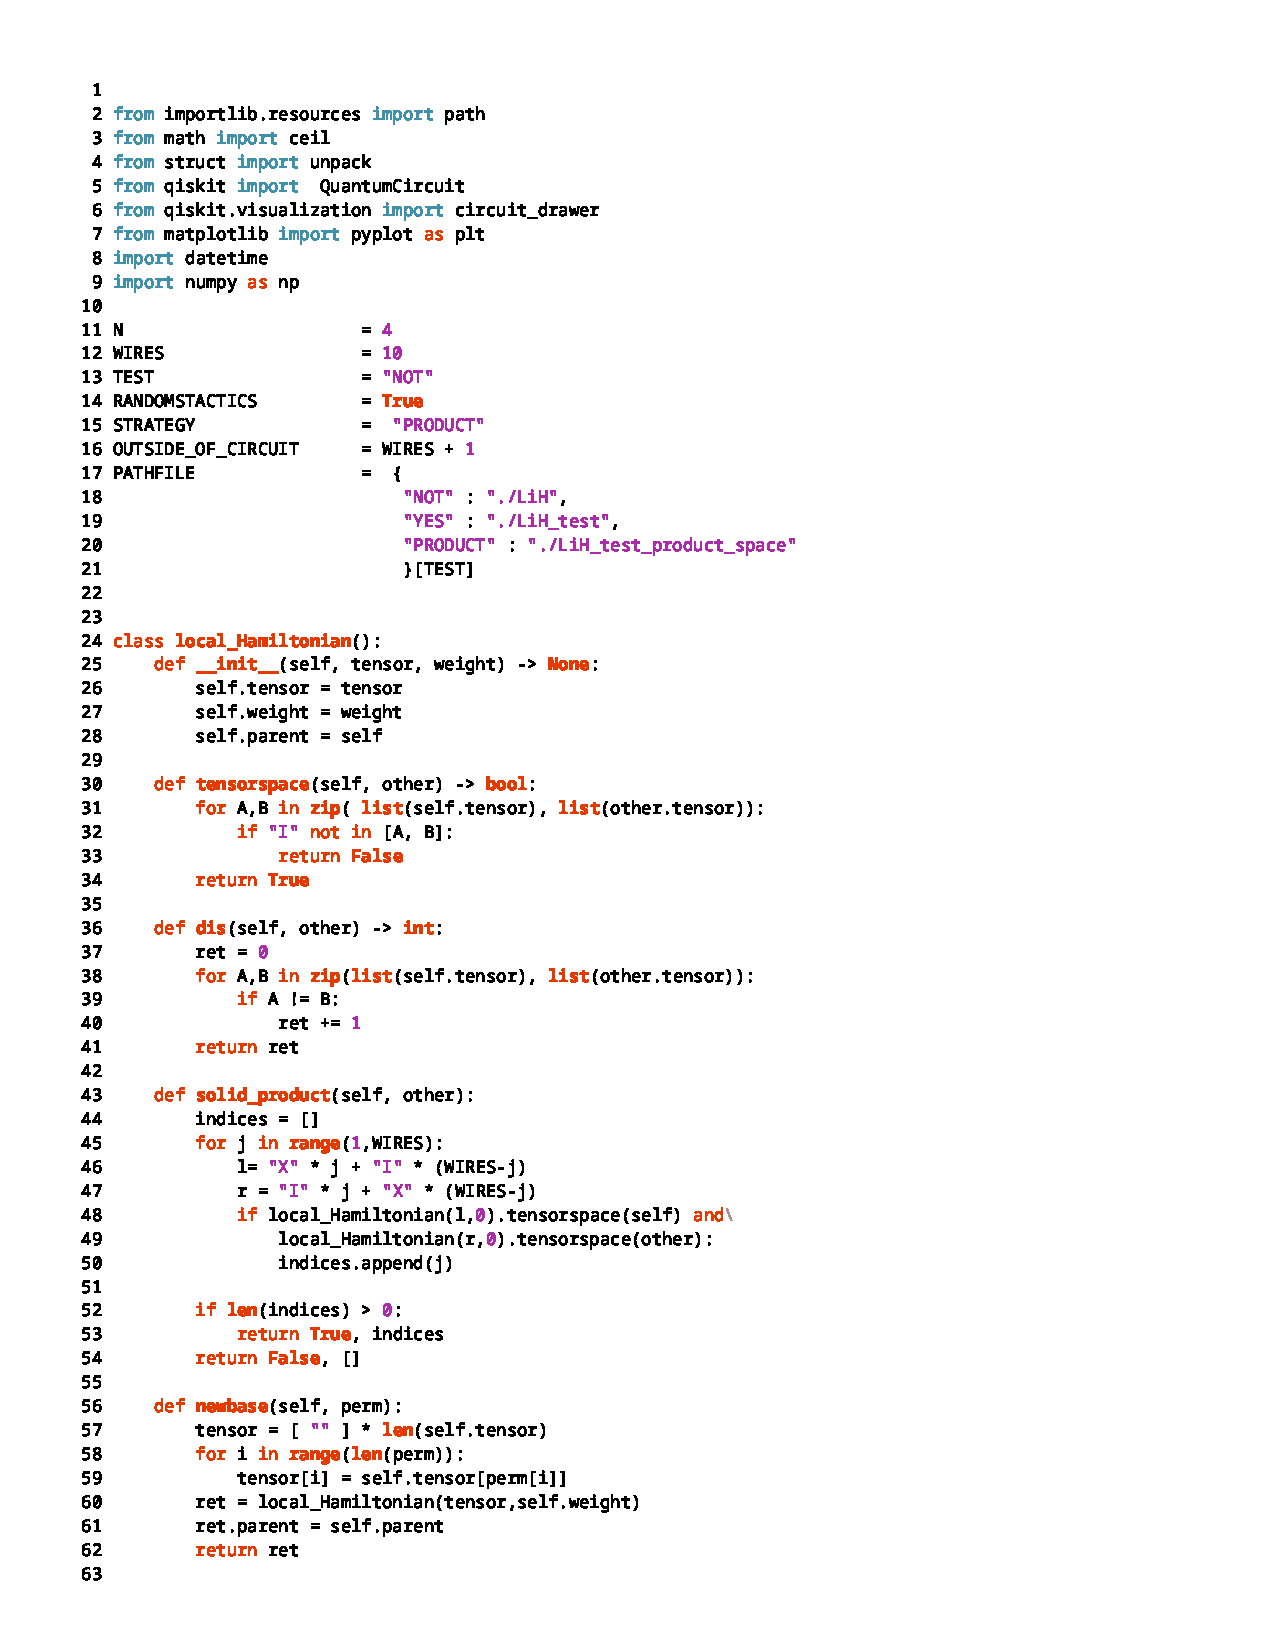
\includepdf[pages=-]{sourcecode.pdf}
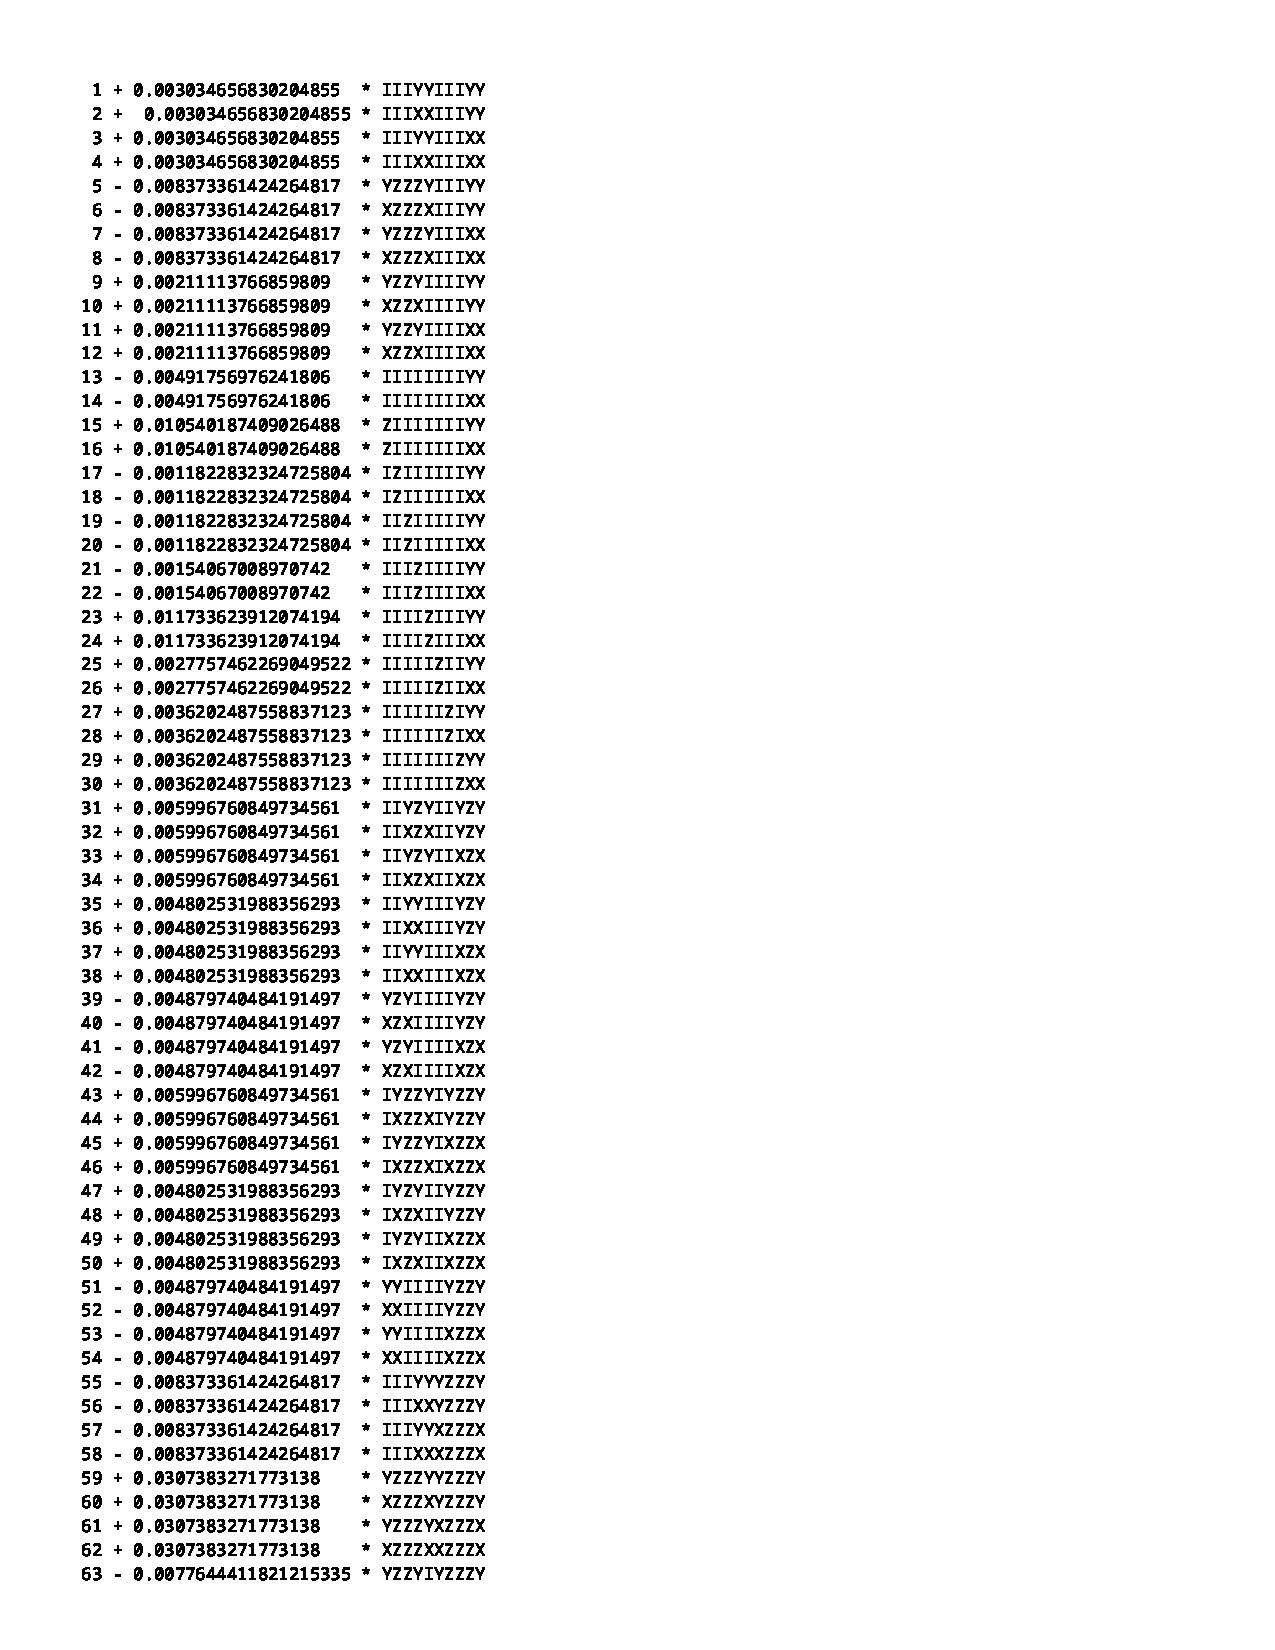
\includepdf[pages=-, link=true]{LiH.html.pdf}
\end{document}
